\documentclass[man, fleqn, noextraspace]{apa6}
\usepackage{lmodern}
\usepackage{amssymb,amsmath}
\usepackage{ifxetex,ifluatex}
\usepackage{fixltx2e} % provides \textsubscript
\ifnum 0\ifxetex 1\fi\ifluatex 1\fi=0 % if pdftex
  \usepackage[T1]{fontenc}
  \usepackage[utf8]{inputenc}
\else % if luatex or xelatex
  \ifxetex
    \usepackage{mathspec}
  \else
    \usepackage{fontspec}
  \fi
  \defaultfontfeatures{Ligatures=TeX,Scale=MatchLowercase}
\fi
% use upquote if available, for straight quotes in verbatim environments
\IfFileExists{upquote.sty}{\usepackage{upquote}}{}
% use microtype if available
\IfFileExists{microtype.sty}{%
\usepackage{microtype}
\UseMicrotypeSet[protrusion]{basicmath} % disable protrusion for tt fonts
}{}
\usepackage{hyperref}
\hypersetup{unicode=true,
            pdftitle={Internet and Social Media Use in American Adults},
            pdfauthor={Cameron S. Kay, Stefania R. Ashby, \& Ashley L. Miller},
            pdfkeywords={american, social media, internet, pew research center},
            pdfborder={0 0 0},
            breaklinks=true}
\urlstyle{same}  % don't use monospace font for urls
\usepackage{graphicx,grffile}
\makeatletter
\def\maxwidth{\ifdim\Gin@nat@width>\linewidth\linewidth\else\Gin@nat@width\fi}
\def\maxheight{\ifdim\Gin@nat@height>\textheight\textheight\else\Gin@nat@height\fi}
\makeatother
% Scale images if necessary, so that they will not overflow the page
% margins by default, and it is still possible to overwrite the defaults
% using explicit options in \includegraphics[width, height, ...]{}
\setkeys{Gin}{width=\maxwidth,height=\maxheight,keepaspectratio}
\IfFileExists{parskip.sty}{%
\usepackage{parskip}
}{% else
\setlength{\parindent}{0pt}
\setlength{\parskip}{6pt plus 2pt minus 1pt}
}
\setlength{\emergencystretch}{3em}  % prevent overfull lines
\providecommand{\tightlist}{%
  \setlength{\itemsep}{0pt}\setlength{\parskip}{0pt}}
\setcounter{secnumdepth}{0}
% Redefines (sub)paragraphs to behave more like sections
\ifx\paragraph\undefined\else
\let\oldparagraph\paragraph
\renewcommand{\paragraph}[1]{\oldparagraph{#1}\mbox{}}
\fi
\ifx\subparagraph\undefined\else
\let\oldsubparagraph\subparagraph
\renewcommand{\subparagraph}[1]{\oldsubparagraph{#1}\mbox{}}
\fi

%%% Use protect on footnotes to avoid problems with footnotes in titles
\let\rmarkdownfootnote\footnote%
\def\footnote{\protect\rmarkdownfootnote}


  \title{Internet and Social Media Use in American Adults}
    \author{Cameron S. Kay\textsuperscript{1}, Stefania R. Ashby\textsuperscript{1},
\& Ashley L. Miller\textsuperscript{1}}
    \date{}
  
\shorttitle{Internet and Social Media}
\affiliation{
\vspace{0.5cm}
\textsuperscript{1} University of Oregon}
\keywords{american, social media, internet, pew research center}
\usepackage{csquotes}
\usepackage{upgreek}
\captionsetup{font=singlespacing,justification=justified}

\usepackage{longtable}
\usepackage{lscape}
\usepackage{multirow}
\usepackage{tabularx}
\usepackage[flushleft]{threeparttable}
\usepackage{threeparttablex}

\newenvironment{lltable}{\begin{landscape}\begin{center}\begin{ThreePartTable}}{\end{ThreePartTable}\end{center}\end{landscape}}

\makeatletter
\newcommand\LastLTentrywidth{1em}
\newlength\longtablewidth
\setlength{\longtablewidth}{1in}
\newcommand{\getlongtablewidth}{\begingroup \ifcsname LT@\roman{LT@tables}\endcsname \global\longtablewidth=0pt \renewcommand{\LT@entry}[2]{\global\advance\longtablewidth by ##2\relax\gdef\LastLTentrywidth{##2}}\@nameuse{LT@\roman{LT@tables}} \fi \endgroup}


\DeclareDelayedFloatFlavor{ThreePartTable}{table}
\DeclareDelayedFloatFlavor{lltable}{table}
\DeclareDelayedFloatFlavor*{longtable}{table}
\makeatletter
\renewcommand{\efloat@iwrite}[1]{\immediate\expandafter\protected@write\csname efloat@post#1\endcsname{}}
\makeatother
\raggedbottom
\setlength{\parskip}{0pt}

\authornote{

Correspondence concerning this article should be addressed to Cameron S.
Kay, 1451 Onyx Street, Eugene, OR 97403. E-mail:
\href{mailto:ckay@uoregon.edu}{\nolinkurl{ckay@uoregon.edu}}}

\abstract{
TBD


}

\usepackage{amsthm}
\newtheorem{theorem}{Theorem}[section]
\newtheorem{lemma}{Lemma}[section]
\theoremstyle{definition}
\newtheorem{definition}{Definition}[section]
\newtheorem{corollary}{Corollary}[section]
\newtheorem{proposition}{Proposition}[section]
\theoremstyle{definition}
\newtheorem{example}{Example}[section]
\theoremstyle{definition}
\newtheorem{exercise}{Exercise}[section]
\theoremstyle{remark}
\newtheorem*{remark}{Remark}
\newtheorem*{solution}{Solution}
\begin{document}
\maketitle

Social media sites are commonly defined as an internet-based service
allowing for the creation and broadcast of user-generated information
(Boyd \& Ellison, 2008; Kaplan \& Haenlein, 2010; Obar \& Wildman,
2015). Obar and Wildman (2015) emphasize the user-generated aspect of
this definition, arguing that this content is the lifeblood of social
media. Although that may sound hyperbolic, it logically follows that if
a site is created with the express purpose of providing user-generated
content, it must have user-generated content to function as intended. By
way of illustration, without videos created by users, YouTube, a social
media site that allows its users to upload and share videos, would fail
to serve its primary purpose. Netflix, a site that allows users to only
stream videos, does not require user-generated content, as it does not
serve user-generated content, and, by extension is not a social media
site. Beyond the functional aspects of social media sites, the
user-generated focus also highlights the importance of individual
differences in the user-service relationship, as users invariably have
characteristics that affect how they consume and generate content.

To explore these individual differences in how people consume and
generate social media content, as well as how they interact with
technology, we conducted secondary data analyses using recent survey
data collected by Pew Research Center (2018).

\section{Method}\label{method}

Survey data examining attitudes towards technology and use of technology
and social media was collected by Pew Research Center (2018). For the
current study, we conducted a secondary data analysis looking at factors
that relate to frequency of social media use, as well as factors that
relate to overall media consumption.

\subsection{Participants}\label{participants}

Two thousand, two people were surveyed by telephone (75.02\% cell phone;
24.98\% landline) over a period of 7 days in January of 2018. We
excluded any participants who reported that they do not even
occasionally use the internet or email (\emph{n} = 273). The resulting
sample comprised 1729 people (45.29\% female). Ages ranged from 18 to 97
(\emph{M} age = 48.29; \emph{SD} age =
17.94)\footnote{Note that the descriptive statistics for age are slightly lower than reality. Ages 97 and older were recorded as simply 97 in the data.}.
Concerning race, 68.48\% identified as white, 12.78\% identified as
black, 3.64\% identified as Asian, 2.95\% identified as mixed race, and
12.15\% refused to answer or reported being from some other race.

\subsection{Materials and Procedure}\label{materials-and-procedure}

Research personnel were instructed to read from a script while
interviewing each participant. For landline users, the script began as
follows:

\enquote{Hello, I am \_\_\_\_\_ calling on behalf of the Pew Research
Center. We are conducting a telephone opinion survey about some
important issues today and we would like to include your household. May
I please speak with the YOUNGEST {[}RANDOMIZE: (MALE / FEMALE){]}, age
18 or older, who is now at home? {[}IF NO MALE/FEMALE, ASK: May I please
speak with the YOUNGEST (FEMALE / MALE), age 18 or older, who is now at
home?{]}}

For cell phone users, the script was slightly different:

\enquote{Hello, I am \_\_\_\_\_ calling on behalf of the Pew Research
Center. We are conducting a telephone opinion survey about some
important issues today. I know I am calling you on a cell phone. If you
would like to be reimbursed for your cell phone minutes, we will pay all
eligible respondents \$5 for participating in this survey. This is NOT a
sales call.}

Once participants passed initial screening (e.g., 18 years of age or
older) and provided verbal consent to the interview, they were asked a
series of questions pertaining to internet use (e.g., \enquote{How often
do you use the internet?}; options ranged from 1 = \enquote{Almost
Constantly} to 5 = \enquote{Less Often}), social media use (e.g.,
\enquote{Do you use any of the following social media sites online or on
your cell phone: Twitter, Instagram, Facebook, Snapchat, YouTube,
WhatsApp, Interest, and LinkedIn?}), as well as perceptions of social
media's influence on the self and society (e.g., \enquote{When you add
up all the advantages and disadvantages of the internet, would you say
the internet has mostly been a good thing or a bad thing for society?};
options included: \enquote{Good Thing}, \enquote{Bad Thing},
\enquote{Some of Both}, and \enquote{Don't Know}). Participants were
also asked about reading habits (e.g., \enquote{During the past 12
months, how many books (print, electronic, and audiobooks) did you read
either all or part of the way through?}) and reading format preferences
(e.g., \enquote{Thinking about all of the books you have read in the
past 12 months, were any of those printed books, audiobooks, or
E-books?}). The interview ended with a series of demographic questions
assessing variables including participant sex, age, race, marrital
status, education, current employment status, income, and political
affiliation.

\subsection{Data analysis}\label{data-analysis}

We used R (Version 3.5.1; R Core Team, 2018) and the R-packages
\emph{bindrcpp} (Version 0.2.2; Müller, 2018), \emph{car} (Version
3.0.0; Fox \& Weisberg, 2011; Fox, Weisberg, \& Price, 2018),
\emph{carData} (Version 3.0.1; Fox et al., 2018), \emph{cowplot}
(Version 0.9.2; Wilke, 2018), \emph{dplyr} (Version 0.7.7; Wickham,
François, Henry, \& Müller, 2018), \emph{emmeans} (Version 1.2.1; Lenth,
2018), \emph{forcats} (Version 0.3.0; Wickham, 2018a), \emph{Formula}
(Version 1.2.3; Zeileis \& Croissant, 2010), \emph{ggplot2} (Version
3.1.0; Wickham, 2016), \emph{here} (Version 0.1; Müller, 2017),
\emph{Hmisc} (Version 4.1.1; Harrell Jr, Charles Dupont, \& others.,
2018), \emph{jcolors} (Version 0.0.4; Huling, 2018), \emph{lattice}
(Version 0.20.35; Sarkar, 2008), \emph{lme4} (Version 1.1.17; Bates,
Mächler, Bolker, \& Walker, 2015), \emph{lmerTest} (Version 3.0.1;
Kuznetsova, Brockhoff, \& Christensen, 2017), \emph{lubridate} (Version
1.7.4; Grolemund \& Wickham, 2011), \emph{magrittr} (Version 1.5; Bache
\& Wickham, 2014), \emph{Matrix} (Version 1.2.14; Bates \& Maechler,
2018), \emph{pander} (Version 0.6.1; Daróczi \& Tsegelskyi, 2018),
\emph{papaja} (Version 0.1.0.9842; Aust \& Barth, 2018), \emph{plotrix}
(Version 3.7.1; J, 2006), \emph{purrr} (Version 0.2.5; Henry \& Wickham,
2018), \emph{readr} (Version 1.2.1; Wickham, Hester, \& Francois, 2017),
\emph{rio} (Version 0.5.10; C.-h. Chan, Chan, Leeper, \& Becker, 2018),
\emph{sjstats} (Version 0.15.0; Lüdecke, 2018), \emph{stringr} (Version
1.3.1; Wickham, 2018b), \emph{survival} (Version 2.42.3; Terry M.
Therneau \& Patricia M. Grambsch, 2000), \emph{tibble} (Version 1.4.2;
Müller \& Wickham, 2018), \emph{tidyr} (Version 0.8.1; Wickham \& Henry,
2018), \emph{tidyverse} (Version 1.2.1; Wickham, 2017), and
\emph{wesanderson} (Version 0.3.6; Ram \& Wickham, 2018) for all our
analyses.

\section{Results}\label{results}

First, we sought to examine how frequency of social media use might vary
as a function of sex, age, social media site, and the interaction
between these variables. Using the \emph{lme4} package by (Bates et al.,
2015), we ran a comparison of seven linear mixed-effects models
predicting frequency of social media use from age, social media site,
sex, and the interactions among these variables. Our first model
included only the random effects. Specifically, we suspected that
participants may have certain response style in evaluating their
frequency of social media use. We entered the subject as a random
intercept to account for interdependence in the participants' ratings.
Although in many cases the scenario or context (i.e., social media site)
would be entered as a random slope, we did not wish to generalize beyond
these sites.

Our second model added gender, followed by age in our third model. The
fourth model included the social media site in question. The fifth
through seventh models added (1) the interaction between sex and age,
(2) the interaction between sex and social media site, and (3) the
interaction between age and social media site.

As shown in Table 1, we found that the addition of age, social media
site, the interaction between sex and social media site, and the
interaction between age and social media site all explained a
significant proportion of variance in social media site usage frequency.
Using the \emph{lmerTest} package from Kuznetsova et al. (2017) to
approximate degrees of freedom with Satterthwaite's method, we found
that older age is associated with lower social media use, \emph{b} =
-0.01, \emph{SE} = .00, \emph{p} \textless{} .003. Furthermore, Snapchat
is used more often than Facebook (\emph{b} = .73, \emph{SE} = .18,
\emph{p} \textless{} .001), and Twitter is used more often than Facebook
(\emph{b} = -0.74, \emph{SE} = .18, \emph{p} \textless{} .001). However,
age interacts with the specific social media site, insofar that
increased age results in even lower rates of social media use in the
case of Instagram (\emph{b} = -0.02, \emph{SE} = .00, \emph{p}
\textless{} .001), Snapchat (\emph{b} = -0.04, \emph{SE} = .00, \emph{p}
\textless{} .001), Twitter (\emph{b} = -0.01, \emph{SE} = .00, \emph{p}
\textless{} .017), and YouTube (\emph{b} = -0.02, \emph{SE} = .00,
\emph{p} \textless{} .001) when compared to Facebook.

Although the model comparison did not indicate an increase in predictive
ability from the introduction of participant gender, we did find that
males (in comparison to females) reported less frequency of social media
use when using the approximated degrees of freedom, \emph{b} = -0.40,
\emph{SE} = .14, \emph{p} \textless{} .005. When compared to Facebook,
however, men exhibitted a greater frequency of using Twitter (\emph{b} =
.49, \emph{SE} = .12, \emph{p} \textless{} .001) and YouTube (\emph{b} =
.61, \emph{SE} = .09, \emph{p} \textless{} .001) than women did.

A comparison of the full model with random effects to the full model
without random effects, revealed that the random effects explained a
significant proportion of the variance in social media site use,
\(\chi^2\)(1) = 176.01, \emph{p} \textless{} .001. In fact, grouping
ratings by participant explained 21.65\% of the variance in the
frequency of using a social media site. A visual inspection of model
residuals did not suggest non-normality nor heteroscedasticity. We also
quantitively inspected the variables for potential multicollinearity
within the fullest model without the interaction effects. No
multicollinearity was detected (\emph{VIF} = 1.01 - 1.04).

\begin{table}[tbp]
\begin{center}
\begin{threeparttable}
\caption{\label{tab:df_lmer_table}Log likelihood comparison of linear mixed-effects models predicting social network site use from sex, age, and specific social network site.}
\begin{tabular}{lrrrrrlrrrrrlrrrrrlrrrrrlrrrrrlrrrrr}
\toprule
 & \multicolumn{1}{c}{\textit{K}} & \multicolumn{1}{c}{$\chi^2$ \textit{df}} & \multicolumn{1}{c}{Loglik.} & \multicolumn{1}{c}{$\chi^2$} & \multicolumn{1}{c}{\textit{p}}\\
\midrule
Null & 3 &  & -6857.08 &  & \\
Sex & 4 & 1 & -6856.28 & 1.61 & .205\\
Age & 5 & 1 & -6775.08 & 162.39 & <.001\\
SNS & 9 & 4 & -6620.63 & 308.91 & <.001\\
Sex X Age & 10 & 1 & -6620.27 & 0.72 & .396\\
Sex X SNS & 14 & 4 & -6591.10 & 58.32 & <.001\\
Age X SNS & 18 & 4 & -6532.52 & 117.18 & <.001\\
\bottomrule
\addlinespace
\end{tabular}
\begin{tablenotes}[para]
\normalsize{\textit{Note.} Participant \textit{N} = 1541; Social Network Site \textit{N} = 5. Null model includes only the random intercept. SNS = social network site. X indicates an interaction.}
\end{tablenotes}
\end{threeparttable}
\end{center}
\end{table}

We next sought to examine how media consumption may vary as a function
of age as well as media format (i.e.~individuals exclusively using print
media, audiobooks, electronic media or combinations of the three). To
explore this data we used the total number of books read in the past
year as an indicator of media consumption. Survey respondents who
endorsed only using a single type of media format were grouped into
their appropriate format bins. Respondents who endorsed using more than
one type of media format were grouped together into a \enquote{mixed
media} format bin. Next, we calculated the average number of books read,
grouped by age and media format see Figure \ref{fig:fig3}.

\begin{figure}
\centering
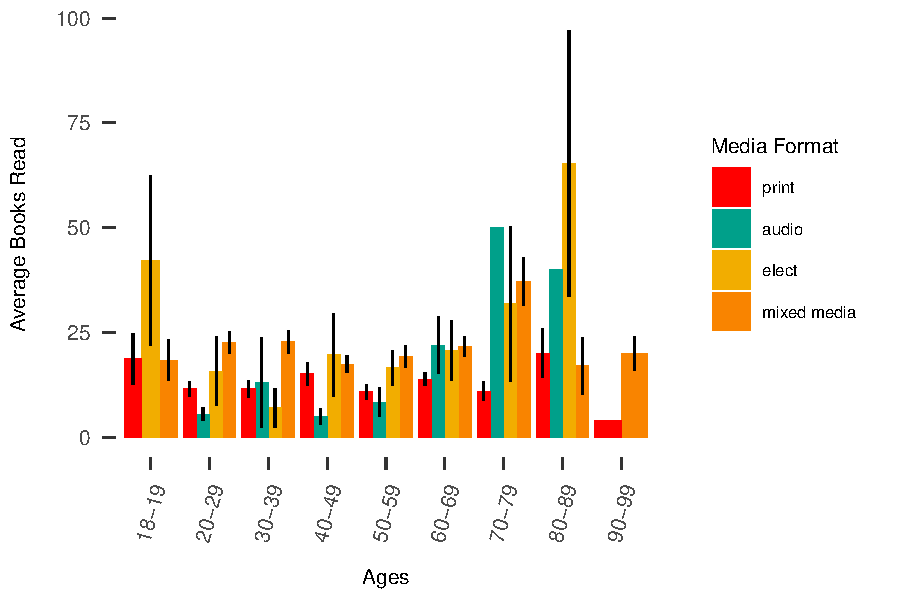
\includegraphics{final_manuscript_files/figure-latex/fig3-1.pdf}
\caption{\label{fig:fig3}Average books read grouped by age and media format}
\end{figure}

To look at the relationships between amount read, age, and media format,
we ran a multiple regression predicting the average number of books read
in the past year from age and media format as well as their interaction.
Results showed a significant main effect of age (STATS) with older
adults reading more books in 2018 than younger adults. We also saw a
significant main effect of media format (STATS) and pairwise comparisons
revealed that books in electronic format were read more than those in
either print and audiobook format. We found no difference in media
consumption between individuals who reported using exclusively a print
format and those who reported using exclusively an audiobook format.
Furthermore, we found no difference between media consumed by
individuals who reported they use mixed media sources compared to those
who exclusively preferred elecronic formats (see Table \ref{tab:reg}.
Figure @ref(fig:fig3

\begin{table}[tbp]
\begin{center}
\begin{threeparttable}
\caption{\label{tab:reg}Main effects of age and media format predicting the average number of books read in 2018.}
\begin{tabular}{llllll}
\toprule
 & \multicolumn{1}{c}{Df} & \multicolumn{1}{c}{Sum Sq} & \multicolumn{1}{c}{Mean Sq} & \multicolumn{1}{c}{F value} & \multicolumn{1}{c}{Pr(>F)}\\
\midrule
age & 1 & 2,165.24 & 2,165.24 & 7.99 & 0.01\\
book\_format & 3 & 5,012.82 & 1,670.94 & 6.17 & 0.00\\
age:book\_format & 3 & 2,124.53 & 708.18 & 2.61 & 0.05\\
Residuals & 200 & 54,193.42 & 270.97 & NA & NA\\
\bottomrule
\end{tabular}
\end{threeparttable}
\end{center}
\end{table}

\begin{figure}
\centering
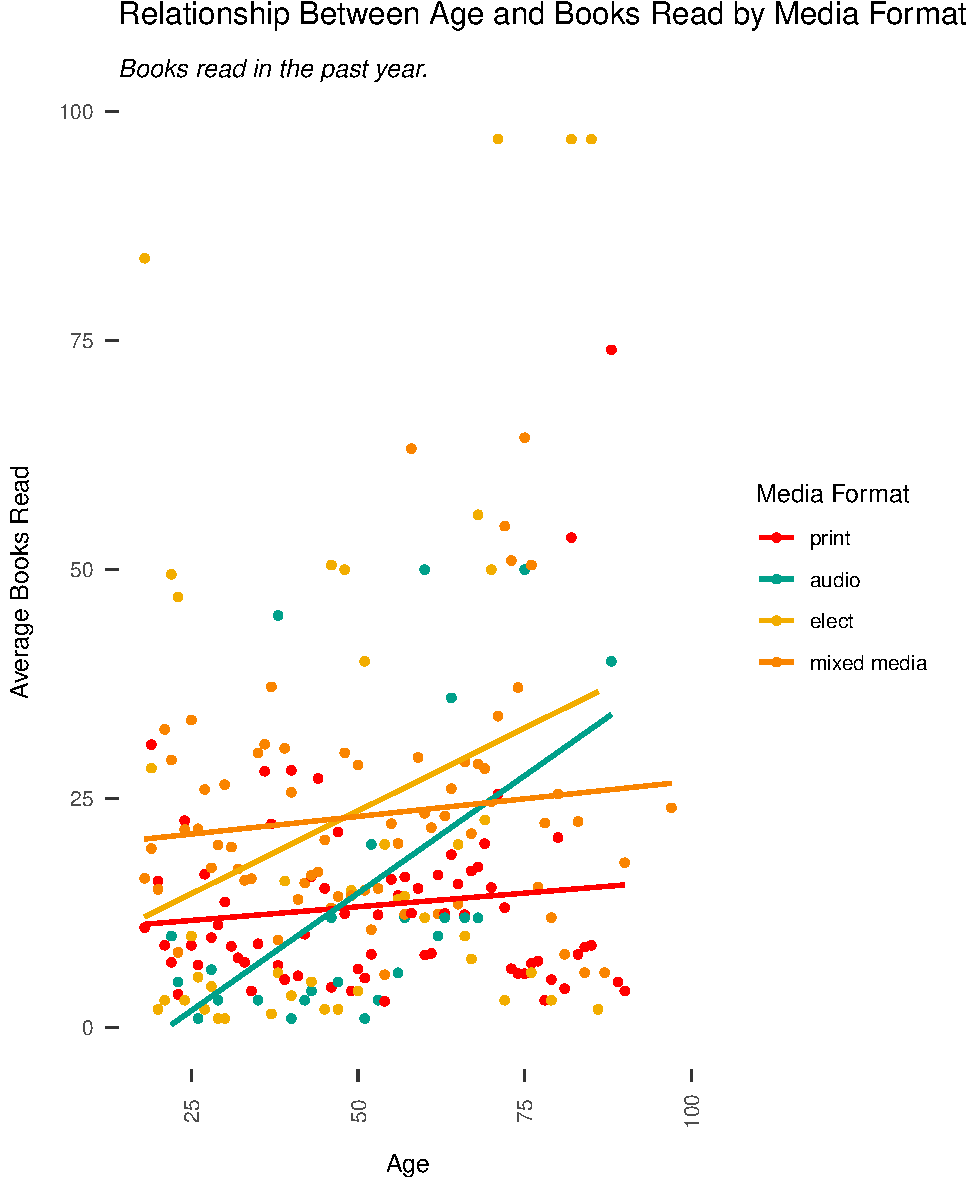
\includegraphics{final_manuscript_files/figure-latex/fig4-1.pdf}
\caption{\label{fig:fig4}Average media consumed as a function of age and
media format}
\end{figure}

\section{Discussion}\label{discussion}

\newpage

\section{References}\label{references}

\begingroup
\setlength{\parindent}{-0.5in} \setlength{\leftskip}{0.5in}

\hypertarget{refs}{}
\hypertarget{ref-R-papaja}{}
Aust, F., \& Barth, M. (2018). \emph{papaja: Create APA manuscripts with
R Markdown}. Retrieved from \url{https://github.com/crsh/papaja}

\hypertarget{ref-R-magrittr}{}
Bache, S. M., \& Wickham, H. (2014). \emph{Magrittr: A forward-pipe
operator for r}. Retrieved from
\url{https://CRAN.R-project.org/package=magrittr}

\hypertarget{ref-R-Matrix}{}
Bates, D., \& Maechler, M. (2018). \emph{Matrix: Sparse and dense matrix
classes and methods}. Retrieved from
\url{https://CRAN.R-project.org/package=Matrix}

\hypertarget{ref-R-lme4}{}
Bates, D., Mächler, M., Bolker, B., \& Walker, S. (2015). Fitting linear
mixed-effects models using lme4. \emph{Journal of Statistical Software},
\emph{67}(1), 1--48.
doi:\href{https://doi.org/10.18637/jss.v067.i01}{10.18637/jss.v067.i01}

\hypertarget{ref-Boyd2008}{}
Boyd, D. M., \& Ellison, N. B. (2008). Social networking sites:
Definitions, history, and scholarship. \emph{Journal of
Computer-Mediated Communication}, \emph{13}, 210--230.

\hypertarget{ref-R-rio}{}
Chan, C.-h., Chan, G. C., Leeper, T. J., \& Becker, J. (2018).
\emph{Rio: A swiss-army knife for data file i/o}.

\hypertarget{ref-R-pander}{}
Daróczi, G., \& Tsegelskyi, R. (2018). \emph{Pander: An r 'pandoc'
writer}. Retrieved from \url{https://CRAN.R-project.org/package=pander}

\hypertarget{ref-R-car}{}
Fox, J., \& Weisberg, S. (2011). \emph{An R companion to applied
regression} (Second.). Thousand Oaks CA: Sage. Retrieved from
\url{http://socserv.socsci.mcmaster.ca/jfox/Books/Companion}

\hypertarget{ref-R-carData}{}
Fox, J., Weisberg, S., \& Price, B. (2018). \emph{CarData: Companion to
applied regression data sets}. Retrieved from
\url{https://CRAN.R-project.org/package=carData}

\hypertarget{ref-R-lubridate}{}
Grolemund, G., \& Wickham, H. (2011). Dates and times made easy with
lubridate. \emph{Journal of Statistical Software}, \emph{40}(3), 1--25.
Retrieved from \url{http://www.jstatsoft.org/v40/i03/}

\hypertarget{ref-R-Hmisc}{}
Harrell Jr, F. E., Charles Dupont, \& others. (2018). \emph{Hmisc:
Harrell miscellaneous}. Retrieved from
\url{https://CRAN.R-project.org/package=Hmisc}

\hypertarget{ref-R-purrr}{}
Henry, L., \& Wickham, H. (2018). \emph{Purrr: Functional programming
tools}. Retrieved from \url{https://CRAN.R-project.org/package=purrr}

\hypertarget{ref-R-jcolors}{}
Huling, J. (2018). \emph{Jcolors: Colors palettes for r and 'ggplot2',
additional themes for 'ggplot2'}. Retrieved from
\url{https://jaredhuling.github.io/jcolors/}

\hypertarget{ref-R-plotrix}{}
J, L. (2006). Plotrix: A package in the red light district of r.
\emph{R-News}, \emph{6}(4), 8--12.

\hypertarget{ref-Kaplan2010}{}
Kaplan, A. M., \& Haenlein, M. (2010). Users of the world, unite! The
challenges and opportunities of Social Media. \emph{Business Horizons},
\emph{53}, 59--68.
doi:\href{https://doi.org/10.1016/j.bushor.2009.09.003}{10.1016/j.bushor.2009.09.003}

\hypertarget{ref-R-lmerTest}{}
Kuznetsova, A., Brockhoff, P. B., \& Christensen, R. H. B. (2017).
lmerTest package: Tests in linear mixed effects models. \emph{Journal of
Statistical Software}, \emph{82}(13), 1--26.
doi:\href{https://doi.org/10.18637/jss.v082.i13}{10.18637/jss.v082.i13}

\hypertarget{ref-R-emmeans}{}
Lenth, R. (2018). \emph{Emmeans: Estimated marginal means, aka
least-squares means}. Retrieved from
\url{https://CRAN.R-project.org/package=emmeans}

\hypertarget{ref-R-sjstats}{}
Lüdecke, D. (2018). \emph{Sjstats: Statistical functions for regression
models (version 0.17.2)}.
doi:\href{https://doi.org/10.5281/zenodo.1284472}{10.5281/zenodo.1284472}

\hypertarget{ref-R-here}{}
Müller, K. (2017). \emph{Here: A simpler way to find your files}.
Retrieved from \url{https://CRAN.R-project.org/package=here}

\hypertarget{ref-R-bindrcpp}{}
Müller, K. (2018). \emph{Bindrcpp: An 'rcpp' interface to active
bindings}. Retrieved from
\url{https://CRAN.R-project.org/package=bindrcpp}

\hypertarget{ref-R-tibble}{}
Müller, K., \& Wickham, H. (2018). \emph{Tibble: Simple data frames}.
Retrieved from \url{https://CRAN.R-project.org/package=tibble}

\hypertarget{ref-Obar2015}{}
Obar, J. A., \& Wildman, S. (2015). Social media definition and the
governance challenge: An introduction to the special issue.
\emph{Telecommunications Policy}, \emph{39}(9), 745--750.

\hypertarget{ref-Pew}{}
Pew Research Center. (2018). Core trends survey. Retrieved from
\url{http://www.pewinternet.org/dataset/jan-3-10-2018-core-trends-survey/}

\hypertarget{ref-R-base}{}
R Core Team. (2018). \emph{R: A language and environment for statistical
computing}. Vienna, Austria: R Foundation for Statistical Computing.
Retrieved from \url{https://www.R-project.org/}

\hypertarget{ref-R-wesanderson}{}
Ram, K., \& Wickham, H. (2018). \emph{Wesanderson: A wes anderson
palette generator}. Retrieved from
\url{https://CRAN.R-project.org/package=wesanderson}

\hypertarget{ref-R-lattice}{}
Sarkar, D. (2008). \emph{Lattice: Multivariate data visualization with
r}. New York: Springer. Retrieved from
\url{http://lmdvr.r-forge.r-project.org}

\hypertarget{ref-R-survival-book}{}
Terry M. Therneau, \& Patricia M. Grambsch. (2000). \emph{Modeling
survival data: Extending the Cox model}. New York: Springer.

\hypertarget{ref-R-ggplot2}{}
Wickham, H. (2016). \emph{Ggplot2: Elegant graphics for data analysis}.
Springer-Verlag New York. Retrieved from \url{http://ggplot2.org}

\hypertarget{ref-R-tidyverse}{}
Wickham, H. (2017). \emph{Tidyverse: Easily install and load the
'tidyverse'}. Retrieved from
\url{https://CRAN.R-project.org/package=tidyverse}

\hypertarget{ref-R-forcats}{}
Wickham, H. (2018a). \emph{Forcats: Tools for working with categorical
variables (factors)}. Retrieved from
\url{https://CRAN.R-project.org/package=forcats}

\hypertarget{ref-R-stringr}{}
Wickham, H. (2018b). \emph{Stringr: Simple, consistent wrappers for
common string operations}. Retrieved from
\url{https://CRAN.R-project.org/package=stringr}

\hypertarget{ref-R-tidyr}{}
Wickham, H., \& Henry, L. (2018). \emph{Tidyr: Easily tidy data with
'spread()' and 'gather()' functions}. Retrieved from
\url{https://CRAN.R-project.org/package=tidyr}

\hypertarget{ref-R-dplyr}{}
Wickham, H., François, R., Henry, L., \& Müller, K. (2018). \emph{Dplyr:
A grammar of data manipulation}. Retrieved from
\url{https://CRAN.R-project.org/package=dplyr}

\hypertarget{ref-R-readr}{}
Wickham, H., Hester, J., \& Francois, R. (2017). \emph{Readr: Read
rectangular text data}. Retrieved from
\url{https://CRAN.R-project.org/package=readr}

\hypertarget{ref-R-cowplot}{}
Wilke, C. O. (2018). \emph{Cowplot: Streamlined plot theme and plot
annotations for 'ggplot2'}. Retrieved from
\url{https://CRAN.R-project.org/package=cowplot}

\hypertarget{ref-R-Formula}{}
Zeileis, A., \& Croissant, Y. (2010). Extended model formulas in R:
Multiple parts and multiple responses. \emph{Journal of Statistical
Software}, \emph{34}(1), 1--13.
doi:\href{https://doi.org/10.18637/jss.v034.i01}{10.18637/jss.v034.i01}

\endgroup


\end{document}
